\chapter{Metodologia}
\label{ch:metodologia}
%Falar porquê do Scrum
%Falar o porquê do Plone

\hspace{2.5cm}

No capítulo de metodologia o objetivo é descrever como ocorreu o processo de construção do sistema, desde a justificativa para a escolha dos métodos de desenvolvimento até a completa entrega do software ao cliente. 

O capítulo está dividido no seguinte escopo: as seções \ref{sec:defMetodologia} e \ref{sec:defCMS} justificam a escolha da metodologia de desenvolvimento e do Sistema de Gerenciamento de Conteúdo para a implementação do sistema, a seção \ref{sec:hospedagem-dominio} apresenta uma análise de custos para contratação de planos de hospedagem e registro de domínio e, por último, a seção \ref{sec:desenvolvimento} apresenta como todas as etapas de implementação e reuniões com o cliente foram estabelecidas.

\hspace{2.5cm}

\section{Definição do tipo de metodologia ágil de desenvolvimento}
\label{sec:defMetodologia}

\hspace{2.5cm}

A definição de uma metodologia ágil de desenvolvimento para o atual projeto é consequência das informações apresentadas na seção \ref{sec:metodologiaagil}, principalmente em relação às informações levantadas nos quadros 1 e 2, que dizem respeito a características das metodologias ágeis e tradicionais, principalmente relativas a tempo, comunicação e riscos tendo em vista a baixa complexidade do projeto, o curto tempo para desenvolvimento e produção da documentação.

Após a certificação de que uma metodologia ágil deve ser empregada, pode-se dizer que vários são os motivos para a escolha do \textit{Scrum} como metodologia de desenvolvimento e \citeonline[~p. 560]{Vasconcelos2015} divulga diversos deles em seu trabalho. Pode-se citar a diminuição de reclamações \apud{mann2005case}{Vasconcelos2015}, o aumento do retorno do investimento em projetos de novos produtos \apud{sulaiman2006agileevm}{Vasconcelos2015}, a melhoria da qualidade do produto produzido e diminuição dos custos de produção \apud{sutherland2008fully}{Vasconcelos2015} e a diminuição no tempo gasto para terminar projetos de desenvolvimento de novos produtos \apud{sanders2007using}{Vasconcelos2015}.

Três características pertencentes ao \textit{Scrum} são a leveza, a simplicidade de entender e a dificuldade de se dominá-lo \apud{sutherland2007scrum}{painka12013utilizaccao}, isto porque é fácil entender suas etapas e o papel de cada um no projeto, mas para adequar essa metodologia à realidade da empresa é necessário experiência e conhecimento.

Assim, às vezes pode ser conveniente alterar prazos, papéis e etapas da metodologia, visando torná-la uma ferramenta de auxílio customizada, e fatores como a disponibilidade de clientes, curtos prazos ou complexidade das tarefas devem interferir em decisões dessa espécie, por isso cada projeto utiliza o \textit{Scrum} de uma maneira, ficando a critério das equipes, em especial o \textit{Scrum Master}, quando e onde remodelar.

Outros fatores que contribuiram para definição do \textit{Scrum} como metodologia de desenvolvimento para o projeto atual estão esclarecidos na tabela 1 e são alusivos ao tamanho da equipe, que corresponde a uma única pessoa, e à elicitação de requisitos, que, por sua vez, não possui uma única forma de ser elaborada. Também contribui para o processo de definição a familiaridade do autor com a metodologia mencionada, já tendo sido estudada e colocada em prática em situações ocorridas durante o curso de Sistemas de Informação.
 
\hspace{2.5cm}
\subsection{Sobre o \textit{Scrum}}
\hspace{2.5cm}

O \textit{Scrum} é um processo para construção incremental de softwares em ambientes complexos e provê o desenvolvimento de softwares em curtas iterações, denominadas \textit{sprints} \citeonline{rising2000scrum}.

\textit{Sprints}: cada \textit{sprint} inclui todas as fases de um software modelo de ciclo de vida de desenvolvimento, como design, implementação, testes, revisão de clientes, etc \cite[~p. 2, tradução nossa]{matharu2015empirical}. Elas têm duração de até 30 dias e também compreendem o procedimento de adaptação a mudança de variáveis (requisitos, tempo, recursos, tecnologia), pois em seu término há sempre uma reflexão sobre as tarefas, definidas antes do início do ciclo, que foram realizadas com sucesso e os próximos incrementos ou revisões as serem executados nas próximas \textit{sprints}, de acordo com o \textit{feedback} passado na reunião com o cliente \citeonline{awad2005comparison}. 

Existem cinco características únicas para o desenvolvimento baseado em \textit{Scrum} \citeonline{matharu2015empirical}, são eles:

\begin{enumerate}
 \item Colaboração: a promoção da colaboração se dá pelo fato do desenvolvimento ser conduzido por equipes compostas por pessoas multifuncionais, envolvendo programadores, arquitetos de software e especialistas em qualidade de software.
 
 \item Encontros diários: são reuniões de curta duração, comandadas pelo \textit{Scrum Master}, onde as equipes de desenvolvimento se comunicam e discutem o progresso com que os requisitos encontrados no \textit{product backlog} estão sendo implementados. \citeonline{rising2000scrum} afirma que esses encontros podem ser realizados três ou quatro vezes na semana e neles os assuntos mais frequentes se baseiam nas dificuldades encontradas e como vencer os obstáculos até a próxima reunião.
 
 \item \textit{Product Backlog}: o \textit{product backlog} captura os requisitos que devem ser implementados, sendo ordenados por nível prioridade. Ele ainda contém erros resolvidos, características gerais e requisitos não funcionais do software.
 
 \item \textit{Sprint Backlog}: este item registra a lista de tarefas que deverão ser realizadas durante a próxima \textit{sprint}. Logicamente a lista de tarefas deve ser baseada no rendimento das equipes para que não haja um planejamento de quantidade de itens exorbitante que dificilmente serão cumpridos. 
 
 \item Regras: são regras fundamentais da metodologia segundo \citeonline{matharu2015empirical}:
 \begin{itemize}
  \item PO \textit{(Product Owner)}: ``responsável pela definição, priorização e comunicação dos requisitos de produto e guias do processo de desenvolvimento'' \cite[~p. 3, tradução nossa]{matharu2015empirical}.
  
  \item Time de desenvolvimento: equipes compostas de 3 a 9 indivíduos responsáveis por executar as tarefas previstas pelo PO.
 
  \item \textit{Scrum Master}: responsável por guiar as equipes no respeito às regras e princípios do \textit{Scrum}. Ele remove impedimentos e auxilia no processo de desenvolvimento.
  
 \end{itemize}
 
\end{enumerate}


Em pesquisa realizada pelo \textit{State of Agile Report} (Estado de Relatório Rápido, em português), em 2019, 72\% das empresas que participaram responderam praticar com \textit{Scrum} ou uma metodologia híbrida que o utiliza como metodologia de desenvolvimento. Tal pesquisa, encontrada em \citeonline{relatorioAnual2019}, foi realizada pela décima terceira vez em 2019 e coletou informações sobre metodologias de processos e desenvolvimento de empresas e organizações da Europa, Ásia, América do Sul e África dos mais variados ramos, tais como de tecnologia, de transporte, industrial, governamental e energético.

Os resultados obtidos com a pesquisa identificam a importância de se conhecer a metodologia estudada nesta seção e como ela ainda é usada por empresas do mundo inteiro. Com o objetivo de assegurar e dar ainda mais veracidade a esta conclusão, outra pesquisa, esta realizada em funcionários da empresa de tecnologia \textit{Microsoft} e via web, detalhada em \citeonline{begel2007usage}, aponta que, das 192 respostas recebidas, a maioria das pessoas que trabalham com desenvolvimento, testes e funções de gerenciamento diretamente ligadas a produção de software aplicam o \textit{Scrum} como a metodologia padrão para construir seus produtos, como representado na figura \ref{ageis-microsoft}. 

\begin{figure}[htb]
 \centering
 \caption{Diferentes metodologias utilizadas pelos funcionários}
 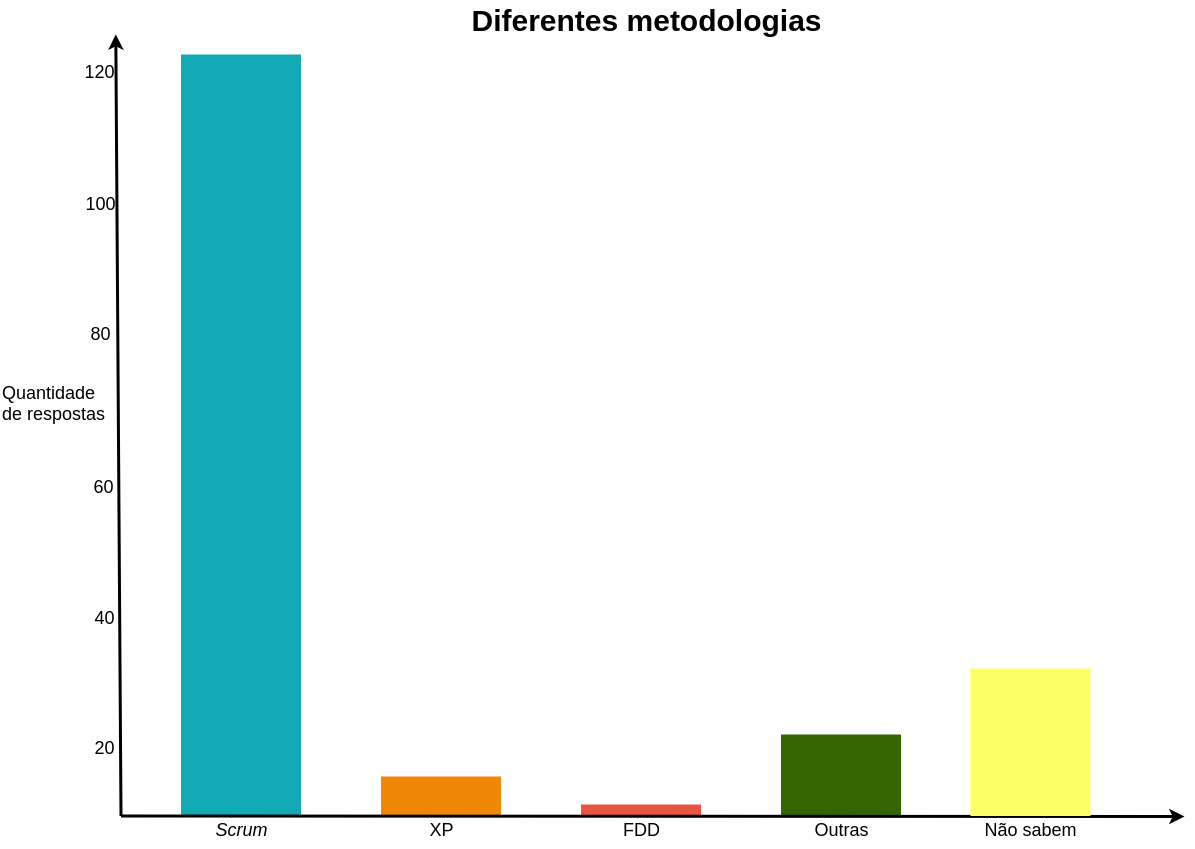
\includegraphics[width=0.8\textwidth]{figuras/diferentes-metodologias}
 \fonte{\citeonline{begel2007usage}. Adaptado.}
 \label{ageis-microsoft}
\end{figure}


\hspace{2.5cm}
\section{Definição do Sistema de Gerenciamento de Conteúdo}
\label{sec:defCMS}

\hspace{2.5cm}

Analisando as informações extraídas na subseção \ref{subsec:comparacao}, no capítulo \ref{ch:referencial}, o sistema para gerenciamento de conteúdo escolhido pelo autor foi o \textit{Plone}. Os principais fatores que influenciaram nesta decisão estão atrelados ao desempenho e segurança de \textit{websites} construídos com esse CMS. Também é importante destacar que o \textit{Plone} é bastante usado para criação de portais, por exemplo o portal da UFVJM, que possuem características semelhantes ao sistema da Kuruatuba, como a publicação de notícias e eventos. 

O \textit{Plone} possui ferramentas personalizadas e de fácil manipulação que facilitam o gerenciamento de notícias e eventos, primeiramente por possuir campos e opções já pré definidos para o tipo de conteúdo que o usuário irá inserir, e por último por inserir automaticamente o conteúdo criado na lista de conteúdos, devido a uma configuração realizada somente uma vez ao criar o sistema. Sendo assim, basta que o usuário preencha os dados relacionados ao tipo de conteúdo (notícia ou evento) para que ele seja criado e já exibido na página web.

Outro ponto positivo do \textit{Plone} é que sua utilização não necessita da instalação de \textit{plug-ins}, extensões ou complementos, podendo ter seus elementos estáticos, como rodapé e cabeçalho, personalizados via \textit{Portlets}, que segundo \citeonline{UFRGS2012}, são aplicativos e ferramentas prontas para uso em qualquer instalação padrão, podendo ser usadas para calendário, notícias, eventos, menu de busca, enquetes, etc. 

\hspace{2.5cm}
\section{Análise de custos sobre hospedagem e domínio}
\label{sec:hospedagem-dominio}
\hspace{2.5cm}

Uma etapa importante na construção de um ou mais sistemas para uma organização sem fins lucrativos é a contratação de serviços de hospedagem e registro de domínio, isto porque é essencial minimizar os custos mantendo, porém, a qualidade desses serviços. Com o propósito de escolher as empresas provedoras dos serviços de hospedagem e registro de domínio, esta seção apresentará um breve comparativo entre os planos de algumas empresas que atuam na prestação desses serviços.

Para o registro de domínio, foram consultados os preços estipulados por quatro das empresas mais conhecidas nesse ramo, são elas: \textit{GoDaddy}, \textit{Hostgator}, \textit{Locaweb} e \textit{Hostinger}. Para o domínio \textit{www.kuruatuba.org}, os valores encontrados estão na tabela \ref{comparativo-dominio}. 

\newpage

\begin{table}[h]
\centering
\scalefont{1.1}
\caption{Preços cobrados pelas empresas para registro do domínio}
\vspace{0.5cm}
\begin{tabular}{l|c}
 
\textbf{Empresa} & \textbf{Valor (R\$/ano)} \\ % Note a separação de col. e a quebra de linhas
\hline                               % para uma linha horizontal
\textit{GoDaddy} & 49,99 \\
\textit{Hostgator} & 49,99 \\
\textit{Locaweb} & 36,90 \\
\textit{Hostinger} & 59 \\

\hline   
\end{tabular}
\fonte{Autor.}
\label{comparativo-dominio}
\end{table}

Como a única variável a ser analisada para a escolha da empresa é o valor cobrado pelo registro, a empresa contratada para registrar o domínio do portal da Kuruatuba foi a \textit{Locaweb}, que elaborou um orçamento com custo inferior às demais. 

A escolha da hospedagem a ser utilizada é possivelmente mais complexa e então necessita uma análise maior por parte do responsável pelo desenvolvimento. Tal complexidade se justifica pela quantidade de variáveis a serem consideradas, como: capacidade de armazenamento e tamanho da largura de banda, e pelo valor médio para contratação de uma VPS, que, por sua vez, é maior que o valor médio de uma hospedagem compartilhada.

Embora haja maior complexidade na análise, algumas opções encontradas no mercado de hospedagem de \textit{websites} foram descartadas rapidamente porque seus planos se aproximam da realidade de empresas maiores, que necessitam utilizar muitos recursos e em alta velocidade tanto para clientes quanto para seus próprios funcionários e estão dispostas a pagar mais pelo serviço. 

Após pesquisas de preços para hopedagem de VPS, foram encontradas duas empresas que possuem um plano básico que se adequa à realidade da Kuruatuba: a \textit{Hostinger} e a \textit{DokeHost}. As especificações ou variáveis consideradas que mais se diferem e importam para a hospedagem do portal e do sistema da Kuruatuba foram as seguintes: capacidade de armazenamento da memória RAM, capacidade de processamento, capacidade de armazenamento da memória secundária e o preço para contratação do serviço. O comparativo das empresas em relação a essas especificações está representada na tabela \ref{comparativo-hospedagem}.

\begin{table}[h]
\centering
\scalefont{0.8}
\caption{Comparativo entre os planos de hospedagem}
\vspace{0.5cm}
\begin{tabular}{l|c|c|c|c}
 
\textbf{Empresa} & \textbf{Memória RAM} & \textbf{vCPU (Quantidade de núcleos)} & \textbf{Memória secundária} & \textbf{Valor (R\$/ano)} \\ % Note a separação de col. e a quebra de linhas
\hline                               % para uma linha horizontal
\textit{Hostinger} & 1GB & 1 & 20GB SSD & 203,88 \\
\textit{DokeHost} & 1GB & 2 & 30GB SSD & 310,80  \\ 

\hline   
\end{tabular}
\fonte{Autor.}
\label{comparativo-hospedagem}
\end{table}

Com o auxílio de uma máquina virtual, foi realizada uma avaliação sobre os prováveis requerimentos mínimos dos sistemas e as especificações ofertadas em cada um dos planos. Após a avaliação, chegou-se à conclusão que provavelmente não será necessário mais que 20GB de armazenamento e muito menos de um processador de 2 núcleos, dada a simplicidade das aplicações a serem hospedadas, não compensando  investir mais de R\$105,00 por ano para tais recursos. Logo, a empresa contratada para a hospedagem das aplicações foi a \textit{Hostinger}.   

\hspace{2.5cm}
\section{Desenvolvimento}
\label{sec:desenvolvimento}

\hspace{2.5cm}
%Definir as etapas 
%Levantamento de requisitos (histórias de usuário) - construção das sprints - Casos de uso e fluxos alternativos

A seção de desenvolvimento sinaliza o início, de fato, da realização das tarefas e demais atividades relacionadas à construção do sistema da Kuruatuba. É a partir desse momento que serão informados dados como domínio, hospedagem, requisitos, versões das tecnologias utilizadas e descrição das atividades desempenhadas.

Para o projeto, foram utilizadas as seguintes ferramentas e suas respectivas versões: \textit{Plone} 4.3.18, PHP 7.4.2, \textit{MySQL} 5.7, \textit{Docker} 19.03.5 e \textit{Git} 2.17.1, este utilizado para o versionamento de código do sistema para cadastro de associados uma vez que ele poderá ser necessário, futuramente, a outro desenvolvedor para atualizações. 

Também é importante mencionar a utilização do \textit{Google Analytics}, que, como já descrito na seção \ref{sec:ferramentas}, possibilita contabilizar número de visitantes e obter informações sobre eles, como: origem, páginas visitadas e tempo por sessão. Outra informação relevante é a utilização das imagens do \textit{Docker}: \textit{robsonggade/lampp-server}, \textit{mysql} e \textit{lmatos/plonebr-zeo}, todas disponíveis no repositório oficial do \textit{Docker}, o \textit{Docker Hub}. 

A escolha da última imagem citada se justifica pela grande customização dos complementos utilizados em portais do governo brasileiro que utilizam a Identidade Digital do Governo (IDG) 2.0, o que facilita muito o trabalho do gerenciador do portal, tornando o \textit{Plone} ainda mais amigável para usuários que desejem adicionar, editar ou excluir elementos rapidamente. Para exemplificar tais complementos pode-se mencionar a capa, que possibilita criar páginas compostas por vários tipos de elementos, sendo muito simples a definição de seu \textit{layout} e inserção dos elementos na mesma.  

A seguir, no decorrer da seção, os temas levantados serão os que se seguem: as subseções \ref{subsec:historias} e \ref{subsec:requisitos} tratarão da elaboração das histórias de usuário e da coleta de requisitos, respectivamente, a subseção \ref{subsec:usecase} apresentará os casos de uso e fluxos alternativos do sistema como forma de auxiliar no entendimento de seu funcionamento, a subseção \ref{subsec:sprints} apresentará como ficaram os elementos do \textit{Scrum} aplicados ao contexto do presente trabalho e, por fim, a estrutura final de \textit{containers} do \textit{Docker} será explicada na subseção \ref{subsec:docker}.

\hspace{2.5cm}
\subsection{Histórias de usuário}
\label{subsec:historias}
\hspace{2.5cm}

Segundo \citeonline{longo2014utilizaccao} as histórias de usuário são muito importantes tanto para a criação de requisitos nos métodos ágeis \textit{Extreme Programming} e \textit{Scrum} quanto para provocar o envolvimento do cliente, porém \citeonline{carvalho2014proposta} ressaltam que elas não poderão substituir a comunicação entre clientes e equipe.

Cada história de usuário deve conter três expressões: ``como um... '', que identifica o papel do usuário na história; ``eu quero...'', funcionalidades requisitadas; e ``de modo que...'', benefício conquistado ao realizar a tarefa \apud{cohn2004user}{longo2014utilizaccao}; além de seis atributos indispensáveis identificados pelo acrônimo inglês INVEST (\textit{Independent, Negotiable, Valuable to users or customers, Estimatable, Small and Testable}) \cite{cohn2004user} e explicados em \citeonline{carvalho2014proposta}:

\begin{itemize}
 \item Independente: uma história deve poder ser desenvolvida, testada e entregue de forma isolada, uma não depende de outras;
 
 \item Negociável: através das histórias é possível discutir requisitos, e por elas ainda deve haver possibilidade de mudanças de funcionalidades e datas de entrega; 
 
 \item Valoroso: assim como os métodos ágeis as histórias de usuário devem proporcionar valor para o cliente, através delas é importante que sinta satisfação e sentimento de realização com as informações discutidas;
 
 \item Estimável: uma equipe deve ser capaz de definir o nível de complexidade, a mão de obra necessária e o tempo para conseguir implementar uma história de usuário. Caso isso não seja possível a história deve ser dividida em histórias menores até que a estimativa seja validada.
 
 \item Tamanho pequeno: as histórias devem ser pequenas para prover maior agilidade na implementação.
 
 \item Testável: testes devem ser realizados em cada história criada pois além dos conteúdos ficarem mais organizados a equipe também conseguirá codificar cada uma caso os testes sejam aceitos.
 
\end{itemize}

A seguir estão as histórias de usuário para o trabalho em questão já testadas e validadas junto ao cliente, uma observação a ser feita corresponde ao fato de que os nomes utilizados nas histórias são fictícios, não fazendo alusão ou referência a nenhum dos envolvidos.

\textbf{História 1}: Como o presidente da associação, João deseja cadastrar e remover, via computador ou \textit{smartphone}, usuários do sistema que vão contribuir nas divulgações e no gerenciamento de associados, de modo a estabelecer possíveis trocas de contribuidores.

\textbf{História 2}: Como presidente da associação, João também deseja publicar, via computador ou \textit{smartphone}, eventos e notícias e alterar o conteúdo estático das páginas quando for necessário, com o objetivo de executar tais tarefas sem necessitar de outro encarregado a prestar tais serviços.

\textbf{História 3}: Como presidente da associação, João precisa gerenciar, via computador ou \textit{smartphone}, o cadastramento de associados, possibilitando o cadastro, a edição, a remoção, a pesquisa e o fornecimento de carteirinha associativa aos mesmos, com o objetivo de adiantar a realização de tarefas sem necessitar de seus subordinados ou responder à solicitação de colaboradores ou visitantes.

\textbf{História 4}: Como um secretário da associação, Paulo pretende publicar, via computador ou \textit{smartphone}, eventos e notícias e alterar o conteúdo de páginas conforme solicitação de seu superior. 

\textbf{História 5}: Como uma secretária da associação, Maria pretende gerenciar, via computador ou \textit{smartphone}, o cadastramento de associados, possibilitando o cadastro, a edição, a remoção, a pesquisa e o fornecimento de carteirinha associativa aos mesmos de acordo com as solicitações vindas do presidente ou dos próprios associados, no âmbito da geração da carteirinha.

\hspace{2.5cm}
\subsection{Coleta de requisitos}
\label{subsec:requisitos}
\hspace{2.5cm}

Uma etapa extremamente importante no desenvolvimento de produtos é a coleta de requisitos, pois é com base nela que artefato será construído, tendo em vista que este é o momento em que o cliente tenta exprimir o que deseja que o software tenha e seja capaz de processar, envolvendo também a abstração dessas informações pela equipe responsável por passá-las para o desenvolvimento. 

Para que tudo ocorra da melhor maneira a qualidade na comunicação é essencial e uma abordagem superficial das ideias deve ser evitada a fim de eliminar falsas convicções, ideias distintas entre cliente e desenvolvedor e desperdício de tempo e demais recursos. Para isso existem as maneiras de extrair os requisitos de sistema do cliente e usuário, como explanado no tópico de especificação de software, na seção \ref{sec:engenhariaweb}. Dentre as opções lá citadas e as histórias de usuário particularizadas na subseção \ref{subsec:historias}, a coleta de requisitos para a aplicação web da Kuruatuba consistiu-se em um formulário e em curtas reuniões com o atual presidente da associação, o professor Erinaldo. 

O formulário, disponibilizado no apêndice \ref{ch:coleta-requisitos}, foi acessível para os futuros utilizadores do sistema para que opinassem sobre o que deveria e o que não deveria estar no produto final, além do grau de importância de cada requisito de acordo com suas exigências e necessidades. De acordo com as respostas registradas no formulário, com reuniões anteriormente mencionadas e com as histórias de usuário descritas obteve-se os seguintes requisitos de sistema:

\begin{enumerate}
 \item Sistema de \textit{login} e cadastro para os usuários;
 \item Publicação de notícias, eventos e mais informações sobre a associação;
 \item Cadastro, atualização e remoção de associados;
 \item Sistema para gerar carteirinha para associados;
 \item Formulário para receber mensagens dos visitantes;
 \item Publicação de eventos organizados pela associação;
 \item \textit{Link} para baixar importantes documentos da Kuruatuba.
\end{enumerate}


\hspace{2.5cm}
\subsection{Casos de uso e fluxos de eventos}
\label{subsec:usecase}
\hspace{2.5cm}

A presente subseção está dividida em duas partes: a primeira, exposta em \ref{subsubsec:casos-uso}, aborda de maneira geral sobre diagramas de casos de uso e apresenta o diagrama associado ao trabalho em desenvolvimento; e a segunda, encontrada em \ref{subsubsec:fluxos}, demonstra a versão final dos fluxos de eventos dos casos de uso.

\hspace{2.5cm}
\subsubsection{Diagrama de casos de uso}
\label{subsubsec:casos-uso}
\hspace{2.5cm}

O diagrama de casos de uso pertence à Linguagem de Modelagem Unificada (UML) e é comumente utilizado para documentar requisitos de sistema, modelando seu contexto e facilitando seu entendimento por exibí-lo externamente aos desenvolvedores \citeonline{de2001diagramas}.

Em geral, os diagramas de casos de uso apresentam os seguintes elementos \citeonline{zapata2007conversion}:

\begin{itemize}
 \item Casos de uso: ações realizadas pelos atores associados que descrevem do início ao fim do processo;
 \item Atores: são os usuários, sendo humanos ou outros sistemas, que poderão realizar os casos de uso e as funcionalidades do sistema;
 \item Relacionamentos: são interações entre dois casos de uso, dois atores ou um caso de uso e um ator. Elas podem der divididas em quatro tipos:
 
 \begin{enumerate}
  \item Associação: estabelece relação entre um ator e um caso de uso;
  \item \textit{include}: inclui o comportamento de um caso de uso em outro, ou seja, ao realizar um caso de uso o outro ligado por meio do \textit{include} também será realizado;
  \item \textit{extend}: a presença do \textit{extend} ligando um caso de uso A a um caso de uso B significa que através de A o \textit{use case} B poderá ser realizado também. Diferentemente do relacionamento anterior, um caso de uso não é obrigatoriamente executado quando o outro for, tal ocorrência se dará por meio de condições;
  \item Herança: este relacionamento simboliza o compartilhamento das especificações de um ator a outro, ou seja, um ator irá herdar todas as permissões em realizar os casos de uso do outro relacionado.
 \end{enumerate}
 
\item Cenário: uma sequência de ações que ilustra um comportamento. São usados para ilustrar a interação ou execução de uma instância a um caso de uso \cite[~p. 239, tradução nossa]{zapata2007conversion}. 

\end{itemize}

Após a breve explicação sobre os diagramas de casos de uso, sua importância e seus elementos, fica representado na figura \ref{use-case} o diagrama referente ao sistema da associação Kuruatuba. Na referida figura está presente a seguinte sigla: CRUD, que, segundo o site \citeonline{devmedia}, é o acrônimo das palavras \textit{Create}, \textit{Read}, \textit{Update} e \textit{Delete} que significam, respectivamente, criar ou cadastrar, ler ou cunsultar, editar ou atualizar, e excluir ou remover.

\begin{figure}[htb]
 \centering
 \caption{Diagrama de casos de uso do sistema da Kuruatuba}
 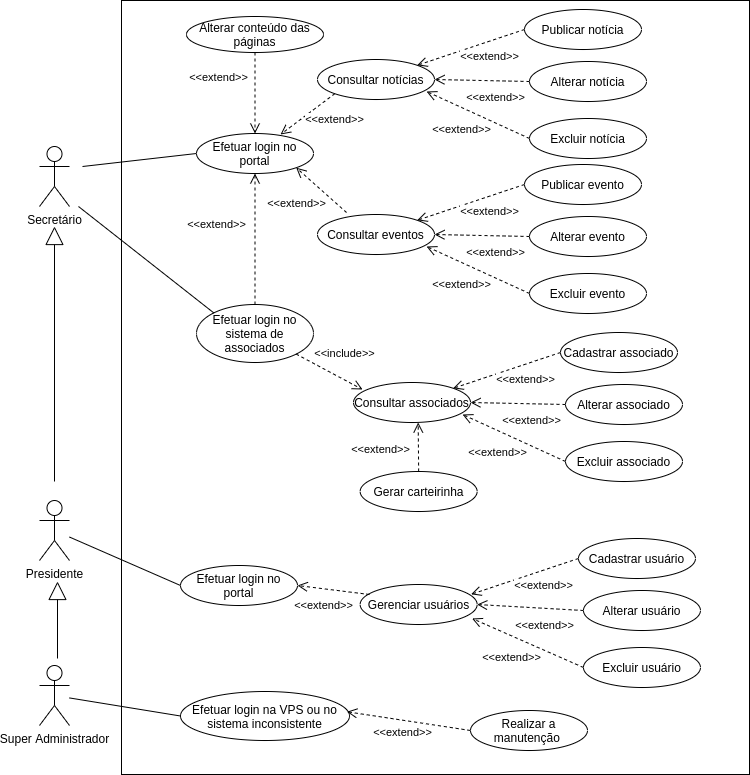
\includegraphics[width=0.8\textwidth]{figuras/use-case-2.png}
 
 \label{use-case}
 \fonte{Autor.}
\end{figure}

\newpage

\hspace{2.5cm}
\subsubsection{Fluxos de eventos}
\label{subsubsec:fluxos}
\hspace{2.5cm}

A seguir estão os fluxos de eventos para os casos de uso definidos anteriormente. Tais fluxos auxiliam ainda mais na compreensão de como o sistema se comportará após cada requisição do usuário e quais possibilidades de interação com a interface do software este terá ao navegar pelas telas.

%login portal
\vspace{0.7cm}
\leftline{ \textbf{Caso de uso}: Efetuar \textit{login} no portal.}

\noindent \textit{Pré-condição}: Inserir o e-mail ou nome de usuário e a senha.

\noindent \textit{Fluxo principal}:

\begin{enumerate}
    \item Ir em ``Acessar'';
    \item inserir os dados de \textit{login};
    \item selecionar o botão ``Acessar'';
    \item O sistema verificará os dados de acesso;
    \item As opções exclusivas ao usuário serão habilitadas.
\end{enumerate}

\noindent \textit{Fluxo alternativo}: Usuário não encontrado.

\noindent \textit{Pré-condição}: dados de \textit{login} inválidos.

\noindent \textit{Etapas}:

\begin{enumerate}
    \item O sistema informa que o usuário ou senha não estão corretos.
\end{enumerate}


%criar página
\vspace{0.7cm}
\leftline{ \textbf{Caso de uso}: Criar página.}

\noindent \textit{Pré-condição}: selecionar o botão de salvar.

\noindent \textit{Fluxo principal}:

\begin{enumerate}
    \item Selecionar no menu o item ``Conteúdo'';
    \item selecionar no menu o item ``Adicionar item'';
    \item selecionar o item ``Página'';
    \item preencher obrigatoriamente o título;
    \item selecionar a opção ``Salvar''.
\end{enumerate}

\noindent \textit{Fluxo alternativo}: Cancelamento do cadastro.

\noindent \textit{Pré-condição}: usuário acionou o botão ``Cancelar''.

\noindent \textit{Etapas}:

\begin{enumerate}
    \item Selecionar o botão ``Cancelar'';
    \item o sistema retorna a mensagem: ``Adicionar Novo Item operação cancelada''.
\end{enumerate}

\noindent \textit{Fluxo alternativo}: Não preenchimento do título.

\noindent \textit{Pré-condição}: usuário acionou o botão ``Salvar'' sem ter inserido o título da página.

\noindent \textit{Etapas}:

\begin{enumerate}
    \item Selecionar o botão ``Salvar'';
    \item o sistema retorna a mensagem: ``Existem alguns erros'';
    \item o campo de título apresenta a seguinte mensagem: ``Dado obrigatório não informado''.
\end{enumerate}



%alterar página
\vspace{0.7cm}
\leftline{ \textbf{Caso de uso}: Alterar página.}

\noindent \textit{Pré-condição}: selecionar a página.

\noindent \textit{Fluxo principal}:

\begin{enumerate}
    \item Selecionar no menu o item ``Conteúdo'';
    \item selecionar a página;
    \item selecionar no menu o item ``Edição'';
    \item após realizar as alterações, ir em salvar.
\end{enumerate}

\noindent \textit{Fluxo alternativo}: Cancelamento de alterações.

\noindent \textit{Pré-condição}: usuário acionou o botão ``Cancelar''.

\noindent \textit{Etapas}:

\begin{enumerate}
    \item Selecionar o botão ``Cancelar'';
    \item o sistema retorna a mensagem: ``Edição cancelada''.
\end{enumerate}


%consultar página
\vspace{0.7cm}
\leftline{ \textbf{Caso de uso}: Consultar página.}

\noindent \textit{Pré-condição}: preencher o campo ``Filtrar''.

\noindent \textit{Fluxo principal}:

\begin{enumerate}
    \item Selecionar no menu o item ``Conteúdo'';
    \item pesquisar por qualquer elemento do portal pelo campo ``Filtrar''.
\end{enumerate}

\noindent \textit{Fluxo alternativo}: Não se aplica.



%excluir página
\vspace{0.7cm}
\leftline{ \textbf{Caso de uso}: Excluir página.}

\noindent \textit{Pré-condição}: selecionar a opção de excluir a página.

\noindent \textit{Fluxo principal}:

\begin{enumerate}
    \item Selecionar no menu o item ``Conteúdo'';
    \item selecionar a página;
    \item selecionar no ícone representado por uma lixeira no canto superior da tela;
    \item o sistema emitirá a mensagem: ``Você tem certeza de que deseja excluir os itens selecionados?'';
    \item selecionar o botão de confirmação da ação.
\end{enumerate}

\noindent \textit{Fluxo alternativo}: Cancelamento da exclusão.

\noindent \textit{Pré-condição}: usuário acionou o botão ``Não''.

\noindent \textit{Etapas}:

\begin{enumerate}
    \item Selecionar o botão ``Não''.
\end{enumerate}



%consultar notícias
\vspace{0.7cm}
\leftline{ \textbf{Caso de uso}: Consultar notícias.}

\noindent \textit{Pré-condição}: preencher o campo ``filtrar notícia''.

\noindent \textit{Fluxo principal}:

\begin{enumerate}
    \item Selecionar no menu o item ``Conteúdo'';
    \item selecionar a pasta notícias;
    \item selecionar a pasta do ano da notícia;
    \item pesquisar por notícia pelo campo ``filtrar notícia''.
\end{enumerate}

\noindent \textit{Fluxo alternativo}: Não se aplica.


%cadastrar notícia
\vspace{0.7cm}
\leftline{ \textbf{Caso de uso}: Publicar notícia.}

\noindent \textit{Pré-condição}: selecionar a opção de salvar a notícia.

\noindent \textit{Fluxo principal}:

\begin{enumerate}
    \item Selecionar no menu o item ``Conteúdo'';
    \item selecionar a pasta notícias;
    \item selecionar a pasta do ano da notícia;
    \item selecionar no menu o item ``Adicionar item'';
    \item selecionar o item ``Notícia'';
    \item preencher obrigatoriamente o título;
    \item selecionar a opção ``Salvar'';
    \item selecionar no menu o item ``Estado'';
    \item selecionar a opção ``Publicar''.
\end{enumerate}

\noindent \textit{Fluxo alternativo}: Cancelamento do cadastro.

\noindent \textit{Pré-condição}:  usuário acionou o botão ``Cancelar''.

\noindent \textit{Etapas}:

\begin{enumerate}
    \item Selecionar o botão ``Cancelar'';
    \item o sistema retorna a mensagem: ``Adicionar Novo Item operação cancelada''.
\end{enumerate}

\noindent \textit{Fluxo alternativo}: Não preenchimento do título.

\noindent \textit{Pré-condição}: usuário acionou o botão ``Salvar'' sem ter inserido o título da notícia.

\noindent \textit{Etapas}:

\begin{enumerate}
    \item Selecionar o botão ``Salvar'';
    \item o sistema retorna a mensagem: ``Existem alguns erros'';
    \item o campo de título apresenta a seguinte mensagem: ``Dado obrigatório não informado''.
\end{enumerate}




%editar notícia
\vspace{0.7cm}
\leftline{ \textbf{Caso de uso}: Alterar notícia.}

\noindent \textit{Pré-condição}: selecionar a opção de salvar a notícia.

\noindent \textit{Fluxo principal}:

\begin{enumerate}
    \item Selecionar no menu o item ``Conteúdo'';
    \item selecionar a pasta notícias;
    \item selecionar a pasta do ano da notícia;
    \item selecionar a notícia;
    \item selecionar no menu o item ``Edição''.
\end{enumerate}

\noindent \textit{Fluxo alternativo}: Cancelamento da edição.

\noindent \textit{Pré-condição}: usuário acionou o botão ``Cancelar''.

\noindent \textit{Etapas}:

\begin{enumerate}
    \item Selecionar o botão ``Cancelar'';
    \item o sistema retorna a mensagem: ``Edição cancelada''.
\end{enumerate}

\noindent \textit{Fluxo alternativo}: Não preenchimento do título.

\noindent \textit{Pré-condição}: usuário acionou o botão ``Salvar'' sem ter inserido o título da notícia.

\noindent \textit{Etapas}:

\begin{enumerate}
    \item Selecionar o botão ``Salvar'';
    \item o sistema retorna a mensagem: ``Existem alguns erros'';
    \item o campo de título apresenta a seguinte mensagem: ``Dado obrigatório não informado''.
\end{enumerate}




%excluir notícia
\vspace{0.7cm}
\leftline{ \textbf{Caso de uso}: Excluir notícia.}

\noindent \textit{Pré-condição}: selecionar a opção de excluir a notícia.

\noindent \textit{Fluxo principal}:

\begin{enumerate}
    \item Selecionar no menu o item ``Conteúdo'';
    \item selecionar a pasta notícias;
    \item selecionar a pasta do ano da notícia;
    \item selecionar a notícia;
    \item selecionar no menu o item ``Ações'';
    \item ir em ``Excluir'';
    \item o sistema emitirá a mensagem: ``Você realmente quer apagar este item?'';
    \item selecionar a opção de excluir.
\end{enumerate}

\noindent \textit{Fluxo alternativo}: Cancelamento da exclusão.

\noindent \textit{Pré-condição}: usuário acionou o botão ``Cancelar''.

\noindent \textit{Etapas}:

\begin{enumerate}
    \item Selecionar o botão ``Cancelar''.
\end{enumerate}




%consultar eventos
\vspace{0.7cm}
\leftline{ \textbf{Caso de uso}: Consultar eventos.}

\noindent \textit{Pré-condição}: preencher o campo ``filtrar eventos''.

\noindent \textit{Fluxo principal}:

\begin{enumerate}
    \item Selecionar no menu o item ``Conteúdo'';
    \item selecionar a pasta eventos;
    \item selecionar a pasta do ano do evento;
    \item pesquisar por evento pelo campo ``filtrar evento''.
\end{enumerate}

\noindent \textit{Fluxo alternativo}: Não se aplica.



%cadastrar evento
\vspace{0.7cm}
\leftline{ \textbf{Caso de uso}: Publicar evento.}

\noindent \textit{Pré-condição}: selecionar a opção de salvar o evento.

\noindent \textit{Fluxo principal}:

\begin{enumerate}
    \item Selecionar no menu o item ``Conteúdo'';
    \item selecionar a pasta eventos;
    \item selecionar a pasta do ano do evento;
    \item selecionar no menu o item ``Adicionar item'';
    \item selecionar o item ``Evento'';
    \item preencher obrigatoriamente o título;
    \item selecionar a opção ``Salvar'';
    \item selecionar no menu o item ``Estado'';
    \item selecionar a opção ``Publicar''.
\end{enumerate}

\noindent \textit{Fluxo alternativo}: Cancelamento do cadastro.

\noindent \textit{Pré-condição}:  usuário acionou o botão ``Cancelar''.

\noindent \textit{Etapas}:

\begin{enumerate}
    \item Selecionar o botão ``Cancelar'';
    \item o sistema retorna a mensagem: ``Adicionar Novo Item operação cancelada''.
\end{enumerate}

\noindent \textit{Fluxo alternativo}: Não preenchimento do título.

\noindent \textit{Pré-condição}: usuário acionou o botão ``Salvar'' sem ter inserido o título do evento.

\noindent \textit{Etapas}:

\begin{enumerate}
    \item Selecionar o botão ``Salvar'';
    \item o sistema retorna a mensagem: ``Existem alguns erros'';
    \item o campo de título apresenta a seguinte mensagem: ``Dado obrigatório não informado''.
\end{enumerate}



%editar evento
\vspace{0.7cm}
\leftline{ \textbf{Caso de uso}: Alterar evento.}

\noindent \textit{Pré-condição}: selecionar a opção de salvar o evento.

\noindent \textit{Fluxo principal}:

\begin{enumerate}
    \item Selecionar no menu o item ``Conteúdo'';
    \item selecionar a pasta eventos;
    \item selecionar a pasta do ano do evento;
    \item selecionar o evento;
    \item selecionar no menu o item ``Edição''.
\end{enumerate}

\noindent \textit{Fluxo alternativo}: Cancelamento da edição.

\noindent \textit{Pré-condição}: usuário acionou o botão ``Cancelar''.

\noindent \textit{Etapas}:

\begin{enumerate}
    \item Selecionar o botão ``Cancelar'';
    \item o sistema retorna a mensagem: ``Edição cancelada''.
\end{enumerate}

\noindent \textit{Fluxo alternativo}: Não preenchimento do título.

\noindent \textit{Pré-condição}: usuário acionou o botão ``Salvar'' sem ter inserido o título do evento.

\noindent \textit{Etapas}:

\begin{enumerate}
    \item Selecionar o botão ``Salvar'';
    \item o sistema retorna a mensagem: ``Existem alguns erros'';
    \item o campo de título apresenta a seguinte mensagem: ``Dado obrigatório não informado''.
\end{enumerate}



%excluir evento
\vspace{0.7cm}
\leftline{ \textbf{Caso de uso}: Excluir evento.}

\noindent \textit{Pré-condição}: selecionar a opção de excluir o evento.

\noindent \textit{Fluxo principal}:

\begin{enumerate}
    \item Selecionar no menu o item ``Conteúdo'';
    \item selecionar a pasta eventos;
    \item selecionar a pasta do ano do evento;
    \item selecionar o evento;
    \item selecionar no menu o item ``Ações'';
    \item ir em ``Excluir'';
    \item o sistema emitirá a mensagem: ``Você realmente quer apagar este item?'';
    \item selecionar a opção de excluir.
\end{enumerate}

\noindent \textit{Fluxo alternativo}: Cancelamento da exclusão.

\noindent \textit{Pré-condição}: usuário acionou o botão ``Cancelar''.

\noindent \textit{Etapas}:

\begin{enumerate}
    \item Selecionar o botão ``Cancelar''.
\end{enumerate}



%login associados
\vspace{0.7cm}
\leftline{ \textbf{Caso de uso}: Efetuar \textit{login} no sistema de associados.}

\noindent \textit{Pré-condição}: Inserir o e-mail ou nome de usuário e a senha.

\noindent \textit{Fluxo principal}:

\begin{enumerate}
    \item No portal, selecionar o item ``Associados'';
    \item confirmar a ação;
    \item inserir os dados de \textit{login};
    \item ir em ``\textit{login}'';
    \item o sistema verificará os dados de acesso;
    \item a lista de associados será exibida.
\end{enumerate}

\noindent \textit{Fluxo alternativo}: Usuário não encontrado.

\noindent \textit{Pré-condição}: dados de \textit{login} inválidos.

\noindent \textit{Etapas}:

\begin{enumerate}
    \item O sistema informa que o usuário ou senha não estão corretos.
\end{enumerate}



%consultar associados
\vspace{0.7cm}
\leftline{ \textbf{Caso de uso}: Consultar associados.}

\noindent \textit{Pré-condição}: preencher o campo ``Consultar''.

\noindent \textit{Fluxo principal}:

\begin{enumerate}
    \item Na página inicial do sistema, inserir alguma informação sobre qualquer atributo do usuário;
    \item a medida que o usuário digitar, o sistema retornará, em tempo real, os resultados para busca.
\end{enumerate}

\noindent \textit{Fluxo alternativo}: Não se aplica.




%cadastrar associado
\vspace{0.7cm}
\leftline{ \textbf{Caso de uso}: Cadastrar associado.}

\noindent \textit{Pré-condição}: selecionar a opção de registrar o associado.

\noindent \textit{Fluxo principal}:

\begin{enumerate}
    \item Acionar o botão ``Adicionar Associado'';
    \item preencher nome, identidade, telefone, rua, número e bairro;
    \item selecionar o botão ``Registrar Associado''.
\end{enumerate}

\noindent \textit{Fluxo alternativo}: Cancelamento do cadastro.

\noindent \textit{Pré-condição}: usuário acionou o botão ``Cancelar''.

\noindent \textit{Etapas}:

\begin{enumerate}
    \item Selecionar o botão ``Cancelar''.
\end{enumerate}

\noindent \textit{Fluxo alternativo}: Não preenchimento dos dados obrigatórios.

\noindent \textit{Pré-condição}: usuário acionou o botão ``Salvar'' sem ter inserido os dados obrigatórios.

\noindent \textit{Etapas}:

\begin{enumerate}
    \item Selecionar o botão ``Salvar'';
    \item os campos obrigatórios apresentam a seguinte mensagem: ``Preencha este campo''.
\end{enumerate}




%editar associado
\vspace{0.7cm}
\leftline{ \textbf{Caso de uso}: Alterar associado.}

\noindent \textit{Pré-condição}: selecionar a opção de atualizar o associado.

\noindent \textit{Fluxo principal}:

\begin{enumerate}
    \item Selecionar o ícone de edição na linha do registro a ser atualizado;
    \item editar os campos necessários;
    \item selecionar o botão de atualizar o associado.
\end{enumerate}

\noindent \textit{Fluxo alternativo}: Cancelamento da edição.

\noindent \textit{Pré-condição}: usuário acionou o botão ``Cancelar''.

\noindent \textit{Etapas}:

\begin{enumerate}
    \item Selecionar o botão ``Cancelar''.
\end{enumerate}

\noindent \textit{Fluxo alternativo}: Não preenchimento dos dados obrigatórios.

\noindent \textit{Pré-condição}: usuário acionou o botão ``Salvar'' sem ter inserido os dados obrigatórios.

\noindent \textit{Etapas}:

\begin{enumerate}
    \item Selecionar o botão ``Atualizar Associado'';
    \item os campos obrigatórios apresentam a seguinte mensagem: ``Preencha este campo''.
\end{enumerate}



%excluir associado
\vspace{0.7cm}
\leftline{ \textbf{Caso de uso}: Excluir associado.}

\noindent \textit{Pré-condição}: selecionar a opção de excluir o associado.

\noindent \textit{Fluxo principal}:

\begin{enumerate}
    \item Selecionar o ícone de exclusão na linha do registro a ser atualizado;
    \item o sistema exibirá uma mensagem de confirmação de exclusão;
    \item selecionar o botão ``OK''.
\end{enumerate}

\noindent \textit{Fluxo alternativo}: Cancelamento da exclusão.

\noindent \textit{Pré-condição}: usuário acionou o botão ``Cancelar''.

\noindent \textit{Etapas}:

\begin{enumerate}
    \item Selecionar o botão ``Cancelar''.
\end{enumerate}



%gerar carteirinha
\vspace{0.7cm}
\leftline{ \textbf{Caso de uso}: Gerar carteirinha.}

\noindent \textit{Pré-condição}: selecionar o ícone de geração de carteirinha para o associado.

\noindent \textit{Fluxo principal}:

\begin{enumerate}
    \item Selecionar o ícone de geração de carteirinha para o associado;
    \item realizar o download ou impressão do documento gerado.
\end{enumerate}

\noindent \textit{Fluxo alternativo}: Não se aplica.

%Gerenciar usuários

\vspace{0.7cm}
\leftline{ \textbf{Caso de uso}: Consultar usuários.}

\noindent \textit{Pré-condição}: estar na página de usuários.

\noindent \textit{Fluxo principal}:

\begin{enumerate}
    \item Selecionar no menu o item ``Configuração de site'';
    \item selecionar a opção ``Usuários e grupos''.
\end{enumerate}

\noindent \textit{Fluxo alternativo}: Não se aplica.



%cadastrar usuário
\vspace{0.7cm}
\leftline{ \textbf{Caso de uso}: Cadastrar usuário.}

\noindent \textit{Pré-condição}: selecionar o botão ``Registrar''.

\noindent \textit{Fluxo principal}:

\begin{enumerate}
    \item Selecionar no menu o item ``Configuração de site'';
    \item selecionar a opção ``Usuários e grupos'';
    \item selecionar o botão ``Adicionar Novo Usuário'';
    \item informar, obrigatoriamente, e-mail e nome de usuário;
    \item selecionar o botão de registrar o usuário.
\end{enumerate}

\noindent \textit{Fluxo alternativo}: Não preenchimento de e-mail ou nome de usuário.

\noindent \textit{Pré-condição}: usuário acionou o botão ``Registrar'' sem ter inserido o e-mail ou nome de usuário.

\noindent \textit{Etapas}:

\begin{enumerate}
    \item Selecionar o botão ``Registrar'';
    \item o sistema retorna a mensagem: ``Houve erros'';
    \item os campos de e-mail e usuário apresentam a seguinte mensagem: ``Dado obrigatório não informado''.
\end{enumerate}




%alterar usuário
\vspace{0.7cm}
\leftline{ \textbf{Caso de uso}: Alterar usuário.}

\noindent \textit{Pré-condição}: selecionar o botão ``Salvar''.

\noindent \textit{Fluxo principal}:

\begin{enumerate}
    \item Selecionar no menu o item ``Configuração de site'';
    \item selecionar a opção ``Usuários e grupos'';
    \item preencher o campo ``Busca de Usuários'';
    \item selecionar o nome do usuário requisitado;
    \item preencher substituir as informações dos campos necessários;
    \item acessar o botão de salvar as informações.
\end{enumerate}

\noindent \textit{Fluxo alternativo}: Cancelamento da edição.

\noindent \textit{Pré-condição}: usuário acionou o botão ``Cancelar''.

\noindent \textit{Etapas}:

\begin{enumerate}
    \item Selecionar o botão ``Cancelar'';
    \item sistema exibe a mensagem: ``Alterações canceladas''.
\end{enumerate}

\noindent \textit{Fluxo alternativo}: Não preenchimento do e-mail.

\noindent \textit{Pré-condição}: usuário acionou o botão ``Salvar'' sem ter haver um e-mail inserido.

\noindent \textit{Etapas}:

\begin{enumerate}
    \item O sistema retorna a mensagem: ``Existem alguns erros'';
    \item o campo de e-mail apresenta a seguinte mensagem: ``Dado obrigatório não informado''.
\end{enumerate}



%remover usuário
\vspace{0.7cm}
\leftline{ \textbf{Caso de uso}: Excluir usuário.}

\noindent \textit{Pré-condição}: selecionar o botão ``Salvar''.

\noindent \textit{Fluxo principal}:

\begin{enumerate}
    \item Selecionar no menu o item ``Configuração de site'';
    \item selecionar a opção ``Usuários e grupos'';
    \item preencher o campo ``Busca de Usuários'';
    \item selecionar a caixa ``Remover'' na linha onde se encontra o nome do usuário requisitado;
    \item selecionar o botão de salvar as informações.
\end{enumerate}

\noindent \textit{Fluxo alternativo}: Não se aplica.



%criar site plone
\vspace{0.7cm}
\leftline{ \textbf{Caso de uso}: Criar site \textit{Plone}.}

\noindent \textit{Pré-condição}: acionar o botão ``Criar site \textit{Plone}''.

\noindent \textit{Fluxo principal}:

\begin{enumerate}
    \item Entrar com usuário e senha no painel de administração do \textit{Zope};
    \item selecionar o botão ``Criar um novo site \textit{Plone}'';
    \item inserir o identificador do site, seu título, idioma e fuso horário;
    \item selecionar o botão ``Criar site \textit{Plone}''.
\end{enumerate}

\noindent \textit{Fluxo alternativo}: Não preenchimento do identificador e do título.

\noindent \textit{Pré-condição}: usuário acionou o botão de criação do site sem ter inserido seu título e identificador.

\noindent \textit{Etapas}:

\begin{enumerate}
    \item Selecionar o botão ``Criar site \textit{Plone}'';
    \item o sistema retorna a mensagem: ``Desculpe, mas parece haver um erro…''.
\end{enumerate}


%consultar site plone
\vspace{0.7cm}
\leftline{ \textbf{Caso de uso}: Consultar site \textit{Plone}.}

\noindent \textit{Pré-condição}: entrar com um usuário e senha na plataforma do \textit{Zope}.

\noindent \textit{Fluxo principal}:

\begin{enumerate}
    \item Entrar com usuário e senha no painel de administração do \textit{Zope}.
\end{enumerate}

\noindent \textit{Fluxo alternativo}: Não se aplica.


%alterar site plone
\vspace{0.7cm}
\leftline{ \textbf{Caso de uso}: Alterar site \textit{Plone}.}

\noindent \textit{Pré-condição}: selecionar o nome do site.

\noindent \textit{Fluxo principal}:

\begin{enumerate}
    \item Entrar com usuário e senha no painel de administração do \textit{Zope};
    \item selecionar o nome do site ou ir em ``Ver seu site \textit{Plone}'' caso exista somente um.
\end{enumerate}

\noindent \textit{Fluxo alternativo}: Não se aplica.


%excluir site plone
\vspace{0.7cm}
\leftline{ \textbf{Caso de uso}: Excluir site \textit{Plone}.}

\noindent \textit{Pré-condição}: selecionar o botão ``Delete''.

\noindent \textit{Fluxo principal}:

\begin{enumerate}
    \item Entrar com usuário e senha no painel de administração do \textit{Zope};
    \item selecionar o link ``Interface de Administração '';
    \item marcar a \textit{checkbox} do site;
    \item acionar o botão para deletá-lo.
\end{enumerate}

\noindent \textit{Fluxo alternativo}: Não se aplica.



%enviar mensagem
\vspace{0.7cm}
\leftline{ \textbf{Caso de uso}: Enviar mensagem para a associação.}

\noindent \textit{Pré-condição}: selecionar o botão ``Enviar''.

\noindent \textit{Fluxo principal}:

\begin{enumerate}
    \item Acessar a aba contato;
    \item inserir as informações para a mensagem;
    \item selecionar o botão de envio.
\end{enumerate}

\noindent \textit{Fluxo alternativo}: Não preenchimento do nome, e-mail, assunto ou corpo da mensagem.

\noindent \textit{Pré-condição}: usuário acionou o botão ``Enviar'' sem ter preenchido nome, e-mail, assunto ou texto da mensagem.

\noindent \textit{Etapas}:

\begin{enumerate}
    \item Os campos obrigatórios vazios apresentam a seguinte mensagem: ``Preencha este campo''.
\end{enumerate}



%----Sprints------%
\hspace{2.5cm}
\subsection{Definição das \textit{sprints}}
\label{subsec:sprints}
\hspace{2.5cm}

A presente subseção irá apresentar os ciclos (\textit{sprints}) de desenvolvimento, que estão definidos na tabela \ref{lista-sprints}. É relevante saber que a interface inicial do portal da Kuruatuba e do sistema de associados foram implementados em máquina local para só depois ocorrer a migração da aplicação para o servidor virtual, sendo que para o primeiro foi realizada uma breve pesquisa por \textit{websites} de outras associações, o que auxiliou na definição de informações que devem constar nas páginas web. 

A realização de todas as atividades contou com o apoio do cliente, que compreende todos os associados, presidente e secretários, de maneira indireta, visto que a troca de informações foi intermediada pelo presidente da Kuruatuba, Erinaldo Barbosa.

A tabela \ref{lista-sprints} contém cada uma das tarefas e as organiza por: identificação da \textit{sprint}, tarefas a serem desenvolvidas, nível de prioridade e prazo para desenvolvimento. Para isso, considera-se o nível de prioridade em uma escala de 1 a 5, em que 1 representa pouquíssima prioridade e 5 altíssima prioridade. Após a tabela, encontram-se explicadas as atividades desenvolvidas.

\begin{table}[h]
\centering
\scalefont{0.9}
\caption{\textit{Product Backlog}}
\vspace{0.5cm}
\begin{tabular}{c|c|c|c}
 
\textbf{Nome} & \textbf{Tarefas} & \textbf{Prioridade} & \textbf{Prazo (dias)} \\ % Note a separação de col. e a quebra de linhas
\hline                               % para uma linha horizontal
\textit{Sprint 1} & Criação da interface inicial & 5 & 14  \\
\textit{Sprint 2} & Contratação e configuração do ambiente de desenvolvimento & 5 & 11  \\ %instalação de todos os softwares e criação dos containers
\textit{Sprint 3} & Alteração de endereço IP (Protocolo da Internet) de imagens nos sistemas & 4 & 4  \\
\textit{Sprint 4} & Configuração do banco de dados e sua conexão com o sistema & 4 & 5  \\
\textit{Sprint 5} & Criação do sistema de autenticação com criptografia & 4 & 5  \\
\textit{Sprint 6} & Organização da página inicial do portal & 5 & 7  \\
\textit{Sprint 7} & Inserção de informações nas páginas informativas & 5 & 7  \\ %criação das páginas 'sobre', 'contato', 'equipe' 
\hline
\end{tabular}
\fonte{Autor.}
\label{lista-sprints}
\end{table}

\textbf{\textit{Sprint 1}}:

\textbf{\textit{Sprint 2}}:

\textbf{\textit{Sprint 3}}:

\textbf{\textit{Sprint 4}}:

\textbf{\textit{Sprint 5}}:

\textbf{\textit{Sprint 6}}:

\textbf{\textit{Sprint 7}}:

%apresentação da interface -> prioridade: 5 -> prazo: 30 dias
%criação das páginas de notícias e eventos -> prioridade: 4 -> prazo: 7 dias
%alimentação das páginas que contêm informações sobre a associação -> prioridade: 2 -> prazo: 7 dias
%implementação da geração de carteirinha, criação e conexão com o banco de dados -> prioridade: 5 -> prazo: 7 dias
%criação da tabela de associados e implementação do CRUD no PHP -> prioridade: 4 -> prazo: 10 dias
%criação do design do sistema de associados -> prioridade: 5 -> prazo: 14 dias
%criação da página de contato -> prioridade: 3 -> prazo: 6 dias
%criação do sistema de login na aplicação para associados -> prioridade: 4 -> prazo: 11 dias
%testes de desempenho e segurança em todo o sistema -> prioridade: 5 -> prazo: 14 dias





\hspace{2.5cm}
\subsection{Estrutura de \textit{containers} do sistema}
\label{subsec:docker}
\hspace{2.5cm}

Como o sistema deve gerenciar dois tipos de público, um de associados e outro de usuários, resolveu-se criar três \textit{containers}: um responsável pelo \textit{Plone} que, por sua vez, apresenta o \textit{website} da Kuruatuba para os visitantes; um \textit{container} responsável por comportar o sistema de gerenciamento de associados, desenvolvido na linguagem PHP, que é conhecida como uma linguagem de programação da era da Web 2.0 que permite o desenvolvimento ágil de software do lado do servidor \citeonline{suzumura2008performance}; e um \textit{container} abrigando o banco de dados, construído com a ferramenta \textit{MySQL}, que possui as informações relacionadas aos associados e onde são realizadas as consultas por parte do sistema escrito em PHP.

A criação e comunicação dos \textit{containers} compactua com as vantagens descritas na seção \ref{sec:ferramentas} do capítulo \ref{ch:referencial}, principalmente no que diz respeito à portabilidade e disponibilidade dos recursos. Tais benefícios também se aplicam à segurança, visto que para uma possível invasão ao sistema, é necessário que o invasor conheça o endereço IP e porta de cada \textit{container} e ainda os dados de acesso tanto ao \textit{website} no \textit{Plone} quanto à aplicação destinada a armazenar os dados sobre os associados.   

Outra justificativa para a divisão das aplicações web está na complexidade de manipulação dos SGBDs - Sistema de Gerenciamento de Banco de Dados - não relacionais. Como já apresentado na subseção \ref{subsec:tipos-cms}, no capítulo \ref{ch:referencial}, o \textit{Plone} utiliza o banco de dados não relacional \textit{ZODB}, e o mesmo é bastante complexo quando o desenvolvedor necessita realizar consultas ou inserções a seus objetos, sendo inviável a criação de páginas ou elementos para tal tarefa.  

% \hspace{2.5cm}
% \section{Execução de testes de desempenho}
% \label{sec:testes}
% \hspace{2.5cm}
